\section{Robustness checks and ERA5 details}
\label{app:reanalysis}
\subsection{Sensitivity to comparison scope}
\label{app:subsets}
The following diagnostics reuse the original 17 PDE tasks within the expanded
collection. They retain the trained models, predictions, and fitting cases.
The 14 task data quality subset excludes Poisson II, Cahn Hilliard I, and
Pressure Poisson for the properties described in Appendix~\ref{app:roster}.
A second subset removes Heat II and Burgers, the two tasks whose B8 case
correspondence was established through checkpoint evaluation. Their intersection
contains 12 tasks. Class aggregation normalizes over represented classes.
These retrospective sensitivity checks do not certify solver validity or
provide independent replication.

\begin{table}[h!]
\centering\small\setlength{\tabcolsep}{3pt}
\caption{\textbf{Sensitivity to dataset inclusion.} Each cell gives the PDE
class ratio followed by the dataset ratio. $N$ counts tasks. Library and
baseline refer to retrospective best models after averaging partitions.
Both mixtures use five fitting examples.}
\label{tab:reviewsensitivity}
\resizebox{\linewidth}{!}{\begin{tabular}{lrrrr}
\toprule
Scope & $N$ & Library / baseline & \shortstack[r]{Fitted mixture /\\Selected model} & \shortstack[r]{Inverse error mixture /\\Selected model} \\
\midrule
Diagnostic set & 17 & 0.764 / 0.820 & 0.876 / 0.918 & 0.882 / 0.924 \\
Data quality subset & 14 & 0.747 / 0.810 & 0.873 / 0.900 & 0.875 / 0.908 \\
Without Heat II and Burgers & 15 & 0.790 / 0.865 & 0.872 / 0.935 & 0.872 / 0.940 \\
Intersection & 12 & 0.776 / 0.865 & 0.869 / 0.918 & 0.865 / 0.926 \\
\bottomrule
\end{tabular}
}
\end{table}

Gains over the Selected model persist across these scopes. Superiority to the
best individual library member is less stable. On the 15 task subset, the
fitted mixture has class ratio 0.916 and dataset ratio 1.020 against that
reference, improving under one aggregation and worsening under the other.
The complete subset and budget tables remain in the companion package.

Source hashes also identify identical M8 and M9 prediction archives on Darcy.
These entries do not supply distinct prediction diversity on that dataset.
Their weights can be redistributed without changing a fitted combined field,
while inverse error weighting is affected by duplication because each copy
receives weight before normalization. Effective model count therefore measures
weight concentration over entries, not independent mechanisms. We retain the
evaluated library and disclose this property rather than interpreting those
weights as unique measures of model usefulness.

\subsection{ERA5 protocol and controls}
\label{app:climateprotocol}
\label{app:era5}
All nine library models use ERA5 training inputs disjoint from the ten fitting
pool and seven evaluation inputs \citep{hersbach2020,niu2024}. M8 and M9 use
49 fine training cases for fitting and six for internal validation, with four
coarse predictions per case assembled by the procedure in
Appendix~\ref{app:experts}. The twelve completed baseline entries represent
eleven independent fits because B10 reuses B9, and the training mean provides
a separate control. Ranked baselines B1 to B11 all have scores on the same
seven evaluation cases.

\begin{table}[h!]
\centering\small
\caption{\textbf{ERA5 mixtures and controls at two fitting budgets.} Mean
relative $L^2$ errors in percent. At $K=5$, three fitting selections use subsets
of the same ten case pool. At $K=10$, they repeat the complete pool. Both
budgets reuse the same seven evaluation cases and trained models.}
\label{tab:era5}\begin{tabular}{lrr}
\toprule
Method & $K=5$ & $K=10$ \\
\midrule
Inverse error mixture & 5.8146 & 5.8358 \\
Fitted mixture & 6.4877 & 6.4736 \\
Selected model (POD GP) & 6.7369 & 6.7369 \\
Training mean field & 6.7369 & 6.7369 \\
Uniform mixture & 6.3730 & 6.3730 \\
All pairs FNO & 17.6992 & 17.6992 \\
Fine only FNO & 23.3336 & 23.3336 \\
\bottomrule
\end{tabular}

\end{table}

POD GP is the best library member, but its output is constant across all
17 reserved inputs and matches the training mean to displayed precision.
Every neural library member has higher error. The inverse error mixture
nevertheless improves on that reference, while autoregressive POD GP and
fidelity basis FNO remain more accurate than either mixture
(Table~\ref{tab:baseline_detail}).
Figure~\ref{fig:era5cases} shows that the inverse error mixture improves six
evaluation cases and the fitted mixture improves five. These seven shared
cases do not support a significance claim or independent training replicates.

\begin{figure}[h!]
\centering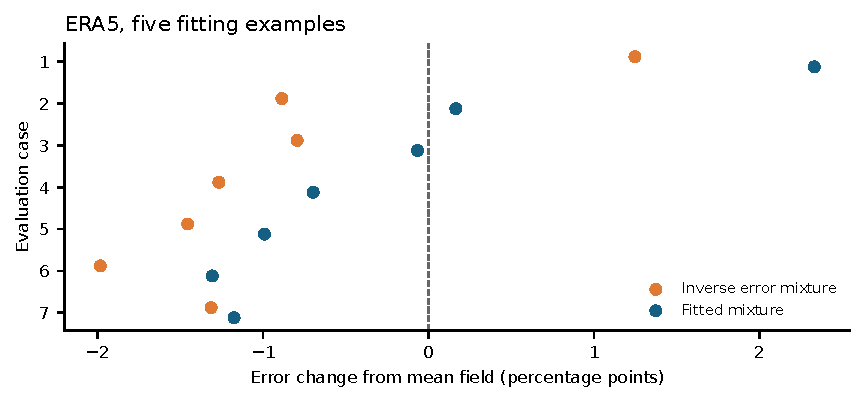
\includegraphics[width=.82\linewidth]{figures/era5_case_errors.pdf}
\caption{\textbf{ERA5 gains by evaluation case.} Change from the training mean
in relative $L^2$ percentage points, averaged over three $K=5$ fitting
selections. Negative values favor the mixture. Case numbers identify archive
rows rather than dates.}
\label{fig:era5cases}
\end{figure}

Predictions and losses use a $128\times256$ working grid, while the native
fine array has $721\times1440$ values. The input variables describe supplied
simulation drivers, not an established forecast origin. Absolute units,
calendar coordinates, and the target transformation remain unverified from
the source arrays. Relative temperature error changes under an additive unit
offset, and the unweighted grid metric is not an area weighted global metric.
These results concern the registered field emulation task, not global climate
skill or operational forecasting.

\subsection{Additional evaluation inputs for Heat I}
\label{app:additionalheat}
This supplementary check uses the existing Heat I library on 40 new fitting
pool cases and 128 new evaluation cases. Three fitting selections share those
evaluation inputs. Table~\ref{tab:fresh} reports the three main rules
separately from the 22 dataset comparison. This single PDE check predates
the direct loss control in Appendix~\ref{app:geometry} and does not establish
generalization to new problem families.

\begin{table}[h!]
\centering\small
\caption{\textbf{Additional Heat I inputs.} Mean relative $L^2$ errors in percent.
Three fitting selections share the same 128 evaluation inputs and trained models.}
\label{tab:fresh}\begin{tabular}{rrrrr}
\toprule
$K$ & \shortstack[r]{Selected\\model} & \shortstack[r]{Inverse\\error\\mixture} & \shortstack[r]{Fitted\\mixture} & All pairs FNO \\
\midrule
5 & 0.008638 & 0.005300 & 0.005454 & 0.011171 \\
10 & 0.008638 & 0.005286 & 0.005359 & 0.011171 \\
20 & 0.008638 & 0.005270 & 0.005296 & 0.011171 \\
\bottomrule
\end{tabular}

\end{table}
